\section{Conclusion}

\subsection{Summary}

\subsection{Future Work}
Because of the rapid development in the fields discussed in this report, much of what we've gone through could be improved in the future. With new \textit{Augmented Reality} and \textit{Mixed Reality} hardware being developed by big franchises, such as Facebook \cite{facebookAR}, the performance will increase ever so rapidly. 
One improvement of our application would be to port it to, not only hand-held devices, but also the headgear, thus allowing the user to building with both hands and never have to pause during the assembly process. 

The model used also only included the pieces to one furniture, but one could easily include more in the future by gathering data for other furniture parts. 

Another issue with our model is that we are unable to detect screws and bolts because of their comparatively small size, instead, we just inform the user that screws should be used during a particular step using animations. This issue could possibly be fixed by adapting our model into taking account to smaller objects.

[SHARED EXPERIENCE IN AR]

\subsubsection{AR stuff}
When working with Augmented Reality it is obviously interesting to know where planes are and how the camera moves in the scene to be able to render virtual object. But usually there is more than one single plane in ones environment. Usually there are other objects in the scene that affects how the virtual objects should be rendered. Sometimes maybe the virtual objects could interact with the real objects to make a more realistic scene. Because of this it can be very interesting to know what those objects actually are.

For example, if you are going to place a virtual furniture in your home it would be good to detect other furnitures in the area so that the virtual object can collide with the real object. This way, they will not intertwine with each other.

% Our master thesis
Or maybe one would like to give virtual instructions to a user for assembling or constructing a certain product or to do maintenance. It is then important to figure out what 3D objects there are in the scene to be able to render instructions on the right places.

Augmented Reality technology has come a long way, but there are still things missing for making it a genuine experience. In ARKit, for instance, if a virtual object is rendered on top of a plane and a real object come in between the virtual object will still be rendered first. This makes it painfully obvious that the virtual object is just a 2D drawing on the screen.

\begin{figure}[hbtp]
\begin{center}
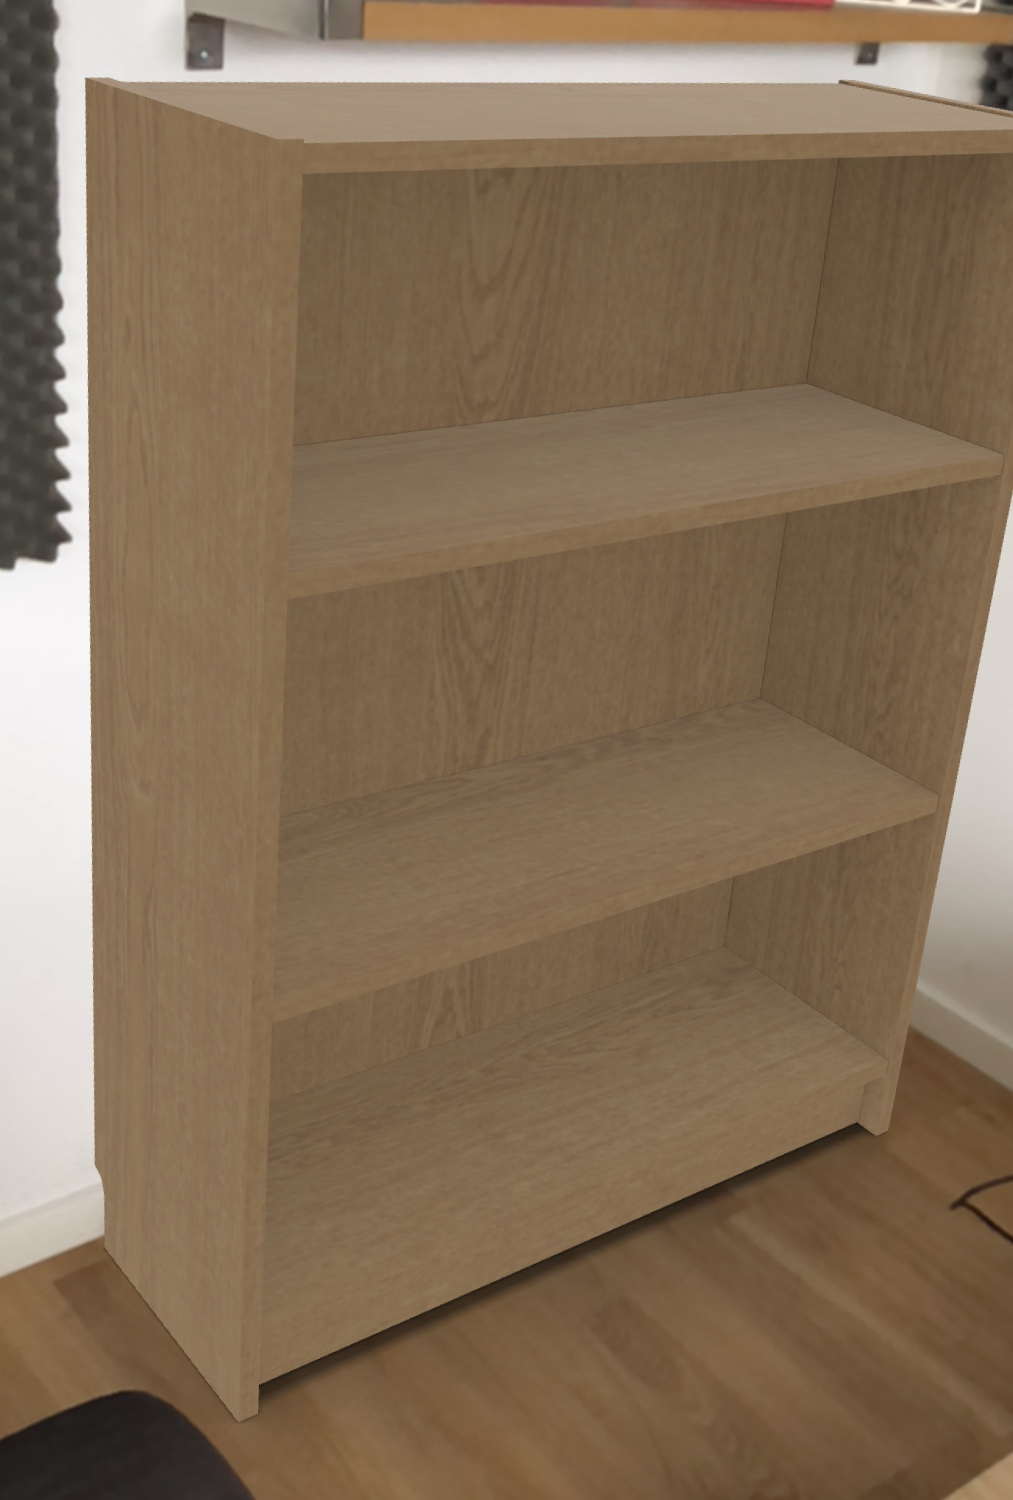
\includegraphics[width = 0.25\textwidth]{./Images/overlapping2.jpg} 
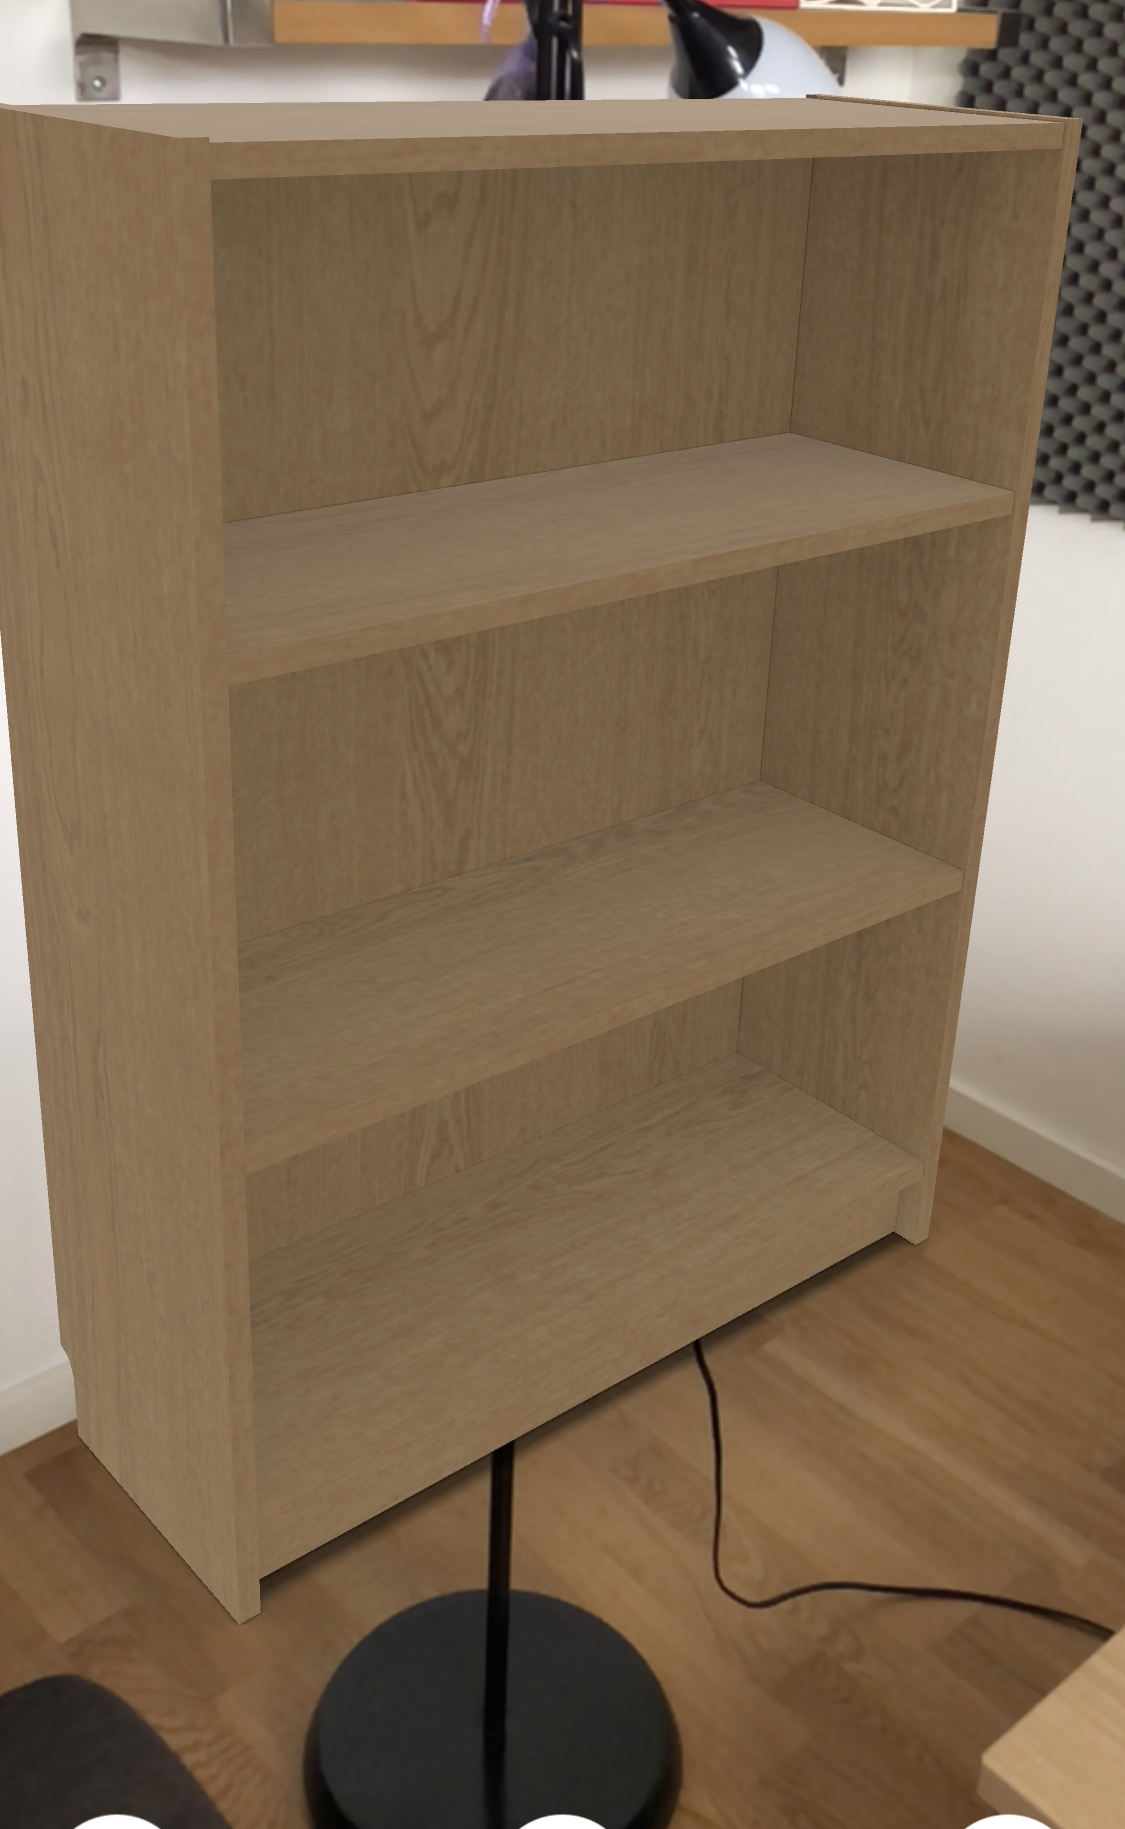
\includegraphics[width = 0.25\textwidth]{./Images/overlapping1.jpg} 
\caption{Book shelf rendered in a corner. To the left no objects in front so it looks realistic.On the right, the book shelf has a lamp in front of it.}
\end{center}
\end{figure}

\newpage